\section{Introduction}
\label{sec:introduction}
A reservoir computer processes a stream of inputs with a fixed dynamical system and trains only a linear
readout~\cite{Maass2002,JaegerESP2001}. In quantum reservoir computing (QRC) the system is
quantum~\cite{Fujii2017}, and the way it keeps and loses information about past inputs decides what it can
compute: recent inputs must stay available, while older inputs and the initial state must fade. Unitary
dynamics does not forget, so dissipation is part of the design~\cite{ChenNurdin2019}. Damping, absorption,
measurement and resets can all create or regulate this fading
memory~\cite{Chen2020,Sannia2024,Ricci2026,Goetting2025,Mujal2023,Franceschetto2026,KobayashiFeedback2024,
Cindrak2024,Sannia2026Memory,Paparelle2026}. Tuning the rate of independent qubit relaxation can improve a
driven spin reservoir~\cite{Sannia2024}, and related work tunes the strengths of the drive, the interactions and
the damping~\cite{MartinezPenaPRL2021,Baumann2026}. In these studies the environment acts as a clock: it sets how fast
the reservoir forgets.

An environment specifies more than a rate. Its jump operators decide which transitions it drives: each qubit
may decay into its own channel, all qubits may decay through one shared channel, pairs may decay together, or
excitations may hop from qubit to qubit. Choosing them is the craft of dissipation engineering, which
prepares and protects quantum states and even computes with
them~\cite{Poyatos1996,Verstraete2009,Pastawski2011,Harrington2022}. A shared channel, for instance, makes
the decay paths of the qubits interfere. Some collective states then decay faster, while others are dark and
do not decay at all, as in subradiance~\cite{Dicke1954,AsenjoGarcia2017,Facchinetti2016}. Earlier QRC studies
tuned the rates of local channels~\cite{Sannia2024}, compared local noise types in gate-based
reservoirs~\cite{Kubota2023,Fry2023}, found that stronger photon loss favours redundant encoding in coupled Kerr
oscillators~\cite{Cheamsawat2025}, or read a static classifier out of a decoherence-free
subspace~\cite{Akshay2026}. How the jump operators themselves shape the memory of a reservoir driven by a time
series has not been compared systematically at equal coupling to the environment.

Here we compare jump families at the same total coupling to the environment (Fig.~\ref{fig:concept}). They
differ in what the environment cannot reach, and this decides how they respond to stronger dissipation. With
separate channels, memory shrinks as the loss grows. With a shared channel it grows: strong loss holds the
reservoir among its dark states by the quantum Zeno effect~\cite{FacchiPascazio2002,Zanardi2014,Burgarth2019},
and the leakage out of them falls as $1/\gamma$. A model of the dark states alone, with nothing fitted,
reproduces the memory of the full reservoir, and erasing the dark coordinates erases it.

Protection has a price. A memory that survives many steps is turned by many later inputs, so an old input
ends up mixed with them (Fig.~\ref{fig:concept}d). We call the number of inputs that a stored function mixes its
order, and we prove that the typical order grows as the mixing fraction of one input times the memory time.
Whether the input can write into the dark states at all is set by the jump operators, and the input amplitude has
to fall as the square root of the leakage to keep the stored signal from shrinking and from mixing. For a
three-spin reservoir we show that this keeps single past inputs readable over a range of delays, the number of past
steps that hold 90\% of the recall, that grows in proportion to the loss rate, though each delay is recalled more
weakly; the memory is carried by coherence between dark states.

Memory here means what a trained linear readout recovers from exact expectation values. The mixing law holds
for a class of reservoirs; the spin results hold in the reservoirs we studied, with specified Hamiltonians and jump
operators. The first version of this study~\cite{BaumannV1} compared the same jump families on four benchmark
tasks (Appendix~\ref{app:v1}) and local with collective relaxation from four to eight spins; the dark-state
mechanism, the mixing law, the writing rule and the proofs are new here.

\begin{figure*}[t]
\centering
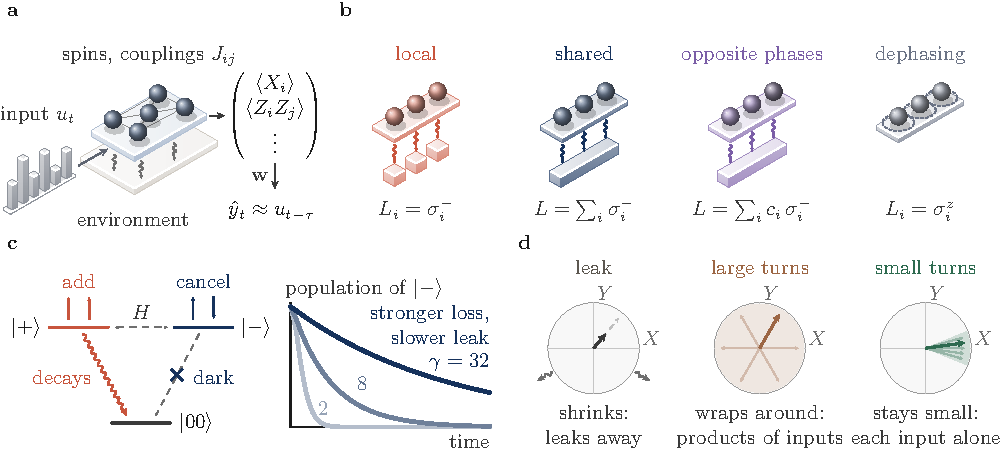
\includegraphics[width=\textwidth]{figures/fig1_concept.pdf}
\caption{\textbf{Engineering the jump operators of a quantum reservoir.}
\textbf{a}~Inputs drive interacting spins coupled to an environment; a linear readout recalls past inputs.
\textbf{b}~Jump families at equal total coupling $\Tr\sum_kL_k^\dagger L_k$, with the number of operators each leaves
untouched (protected) at five spins.
\textbf{c}~Two spins sharing one channel. The decay amplitudes of $|10\rangle$ and $|01\rangle$ add for
$|{+}\rangle$, which decays, and cancel for $|{-}\rangle$, which is dark. The Hamiltonian $H$ mixes the two; strong
loss turns this into a slow leak, so the dark state survives longer the stronger the loss (inset: coupling $g$
between $|{+}\rangle$ and $|{-}\rangle$, $\gamma/g=2$, 8, 32).
\textbf{d}~Each input turns the stored state by $\pm\theta$, so over the memory time its direction spreads by about
$\theta\sqrt{t_{\mathrm{mem}}}$. Small turns keep the spread small and the readout sees each input on its own; large
turns let it wrap around and the readout sees only products of inputs.}
\label{fig:concept}
\end{figure*}
